\documentclass[english]{article}
\usepackage{graphicx}
\usepackage{amsmath}
\usepackage{hyperref}
\usepackage{setspace}
\usepackage{apacite}
\usepackage{natbib}
\usepackage{pxfonts}
\usepackage[utf8]{inputenc}
\usepackage[left=1in,right=1in,top=1in,bottom=1in]{geometry}
\usepackage[left]{lineno}
\usepackage{soul}
\linenumbers


\title{An examination of the high-order dynamic interactions
  underlying multi-dimensional timeseries data} \author{Lucy
  L. W. Owen$^1$, Thomas Hao Chang$^{1,2}$, and\
  Jeremy R. Manning\textsuperscript{$1, \dagger$}\\
  [0.1in]$^1$Department of Psychological and Brain
  Sciences,\\Dartmouth
  College, Hanover, NH\\
  $^3$Amazon.com, Seattle, WA\\
  \textsuperscript{$\dagger$}Address correspondence to
  jeremy.r.manning@dartmouth.edu}


\begin{document}
\maketitle


\begin{abstract}
  Most complex systems reflect dynamic interations between myriad
  evolving components (e.g., interacting molecules, interacting brain
  systems, interacting individuals within a social network or
  ecological system, coordinated components within a mechanical or
  digital device, etc.).  Despite that these interactions are central
  to the full system's behavior (e.g., removing a component from the
  full system can change the entire system's behavior), dynamic
  interactions cannot typically be directly measured.  Rather, the
  interactions must be inferred through their hypothesized role in
  guiding the dynamics of system components.  Here we use a
  model-based approach to inferring dynamic interactions from
  timeseries data.  In addition to examining first-order interactions
  (e.g., between pairs of components) we also examine higher-order
  interactions (e.g., that characterize mirrored structure in the
  patterns of interaction dynamics displayed by different subsets of
  components).  We apply our approach to two datasets.  First, we use
  a synthetic dataset, for which the underlying dynamic interactions
  are known, to show that our model recovers those ground-truth
  dynamic interactions.  We also apply our model to a neuroimaging
  dataset and show that the high-order dynamic interactions exhibited
  by brain data vary meaningfully as a function of the cognitive
  ``richness'' of the stimulus people are experiencing.
\end{abstract}

\doublespacing

\section*{Introduction}
The dynamics of the observable universe are meaningful in three
respects.  First, the behaviors of the \textit{atomic units} that
exhibit those dynamics are highly interrelated.  The actions of one
unit typically have implications for one or more other units.  In
other words, there is non-trivial \textit{correlational structure}
defining how different units interact with and relate to each other.
Second, that correlational structure is \textit{hierarchical} in the
sense that it exists on many spatiotemporal scales.  The way one group
of units interacts may relate to how another group of units interact,
and the interactions between those groups may exhibit some rich
structure.  Third, the structure at each level of this correlational
hierarchy changes from moment to moment, reflecting the ``behavior''
of the full system.

These three properties (rich correlations, hierarchical organization,
and dynamics) are major hallmarks of many complex systems.  For
example, within a single cell, the cellular components interact at
many spatiotemporal scales, and those interactions change according to
what that single cell is doing.  Within a single human brain, the
individual neurons interact within each brain structure, and the
structures interact to form complex networks.  The interactions at
each scale vary according to the functions our brains are carrying
out.  And within social groups, interactions at different scales
(e.g., between individuals, family units, communities, etc.) vary over
time according to changing goals and external constraints.

Although many systems exhibit rich dynamic correlations at many
scales, a major challenge to studying such patterns is that typically
neither the correlations nor the hierarchical organizations of those
correlations may be directly observed.  Rather, these fundamental
properties must be inferred indirectly by examining the observable
parts of the system-- e.g., the behaviors of the individual atomic
units of that system.  In the \textit{Methods} section, we propose a
series of mathematical operations that may be used to recover dynamic
correlations at a range of scales (i.e., orders of interaction).  In
the \textit{Results} section, we demonstrate how our approach may be
applied to multi-dimensional timeseries data: a synthetic dataset
where the underlying dynamic correlations are known (we use this
dataset to validate our approach), and a neuroimaging dataset
comprising data collected as participants listened to a
story~\citep{SimoEtal16}.  In different experimental conditions in the
neuroimaging study, participants listened to altered versions of the
story that varied in cognitive richness: the intact story (fully
engaging), a scrambled version of the story where the paragraphs were
presented in a randomized order (moderately engaging), a second
scrambled condition where the words were presented in a random order
(minimally engaging), and a ``rest'' condition where the participants
did not listen to any version of the story (control condition).  We
use the neuroimaging dataset to examine how higher-order structure in
brain data varies as a function of the cognitive richness of the
stimulus.

\section*{Methods}
There are two basic steps to our approach.  In the first step, we take
a number-of-timepoints ($T$) by number-of-features ($F$)
\textit{matrix of observations} ($\mathbf{X}$) and we return a $T$ by
$\frac{F^2 - F}{2}$ \textit{matrix of dynamic correlations}
($\mathbf{Y}$).  Here $\mathbf{Y_0}$ describes, at each moment, how
all of the features (columns of $\mathbf{X}$) are inferred to be
interacting.  (Since the interactions are assumed to be non-recurrent
and symmetric, only the upper triangle of the full correlation matrix
is computed.)  In the second step, we project $\mathbf{Y_0}$ onto an
$F$-dimensional space, resulting in a new $T$ by $F$ matrix
$\mathbf{Y_1}$.  Note that $\mathbf{Y_1}$ contains information about
the correlation dynamics present in $\mathbf{X}$, but represented in a
compressed number of dimensions.  By repeatedly applying these two
steps in sequence, we can examine and explore higher order dynamic
correlations in $\mathbf{X}$.

\subsection*{Dynamic correlations}
Given a matrix of observations, we can compute the (static)
correlations between any pair of observations, $\mathbf{X}_i$ and
$\mathbf{X}_j$ using:
\begin{align}
  \mathrm{corr}(\mathbf{X}_i, \mathbf{X}_j) &= \frac{\sum_{t=1}^T \left(\mathbf{X}_i(t)
                                              -
                                              \bar{\mathbf{X}_i}\right) \left(\mathbf{X}_j(t)
                                              -
                                              \bar{\mathbf{X}_j}\right)}{\sqrt{\sum_{t=1}^T
                                              \sigma^2_{\mathbf{X}_i} 
                                              \sigma^2_{\mathbf{X}_j}}},~\mathrm{where}\\\label{eqn:corr}
  \bar{\mathbf{X}_k} &= \sum_{t=1}^T
                       \mathbf{X}_k(t),~\mathrm{and}\\
  \sigma^2_{\mathbf{X}_k} &= \sum_{t=1}^T \left( \mathbf{X}_k -
                            \bar{\mathbf{X}_k} \right)^2 
\end{align}

We can generalize this formula to compute time-varying correlations by
incorporating a \textit{weight function} that takes a time $t$ as input,
and returns how much the observed data every timepoint (including $t$)
contribute to the correlations at time $t$ (Fig.~\ref{fig:weights}).
\begin{figure}
  \centering
  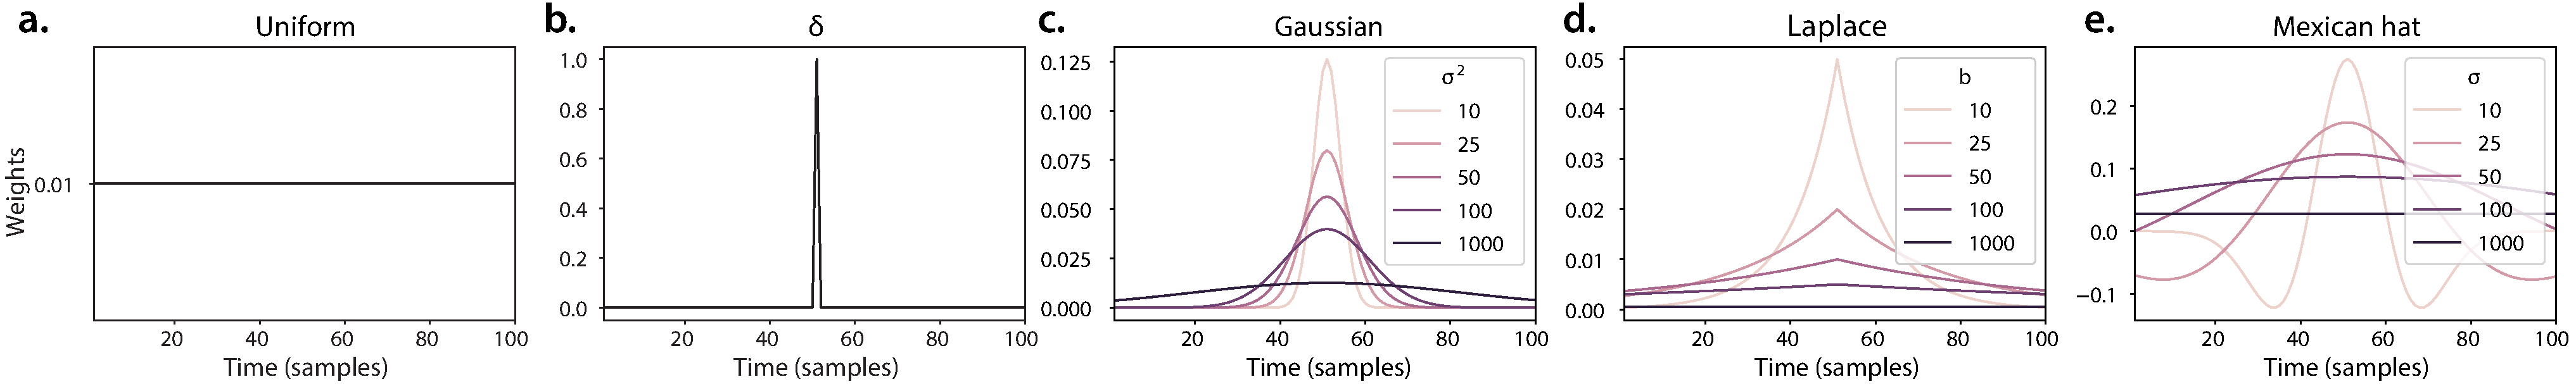
\includegraphics[width=\textwidth]{figs/kernels}
  \caption{\textbf{Examples of time-varying weights.  Each panel
      displays per-timepoint weights at $t = 50$, evaluated for 100
      timepoints ($1, ..., 100$).  a. Uniform weights.} The weights
    are timepoint-invariant; observations at all timepoints are
    weighted equally, and do not change as a function of $t$.  This is
    a special case of weight function that reduces dynamic
    correlations to static correlations.  \textbf{b. Dirac delta
      function.} Only the observation at timepoint $t$ is given weight
    (of 1), and weights for observations at all other timepoints are
    set to 0.  \textbf{c. Gaussian weights.} Each observation's
    weights fall off in time according to a Gaussian probability
    density function centered on $\mu = t$.  Weights derived using
    several different example variance parameters ($\sigma^2$ are
    displayed.  \textbf{d. Laplace weights.}  Each observation's
    weights fall off in time according to a Laplace probability
    density function centered on $\mu = t$.  Weights derived using
    several different example scale parameters ($b$) are displayed.
    \textbf{e. Mexican hat (Ricker wavelet) weights.}  Each
    observation's weights fall off in time according to a Ricker
    wavelet centered on $t$.  This function highlights the
    \textit{contrasts} between local versus surrounding activity
    patterns in estimating dynamic correlations. Weights derived using
    several different example width parameters ($\sigma$) are
    displayed.  }
  \label{fig:weights}
\end{figure}

Given a weight function $w(t)$ for timepoint $t$, evaluated at
timepoints in the interval $\left[ 1, ..., T \right]$, we can extend the static correlation formula
in Equation~\ref{eqn:corr} to reflect an \textit{instantaneous
  correlation} at timepoint $t$:
\begin{align}
  \mathrm{timecorr}(\mathbf{X}_i, \mathbf{X}_j, t) &= \frac{\sum_{t=1}^T \left(\mathbf{X}_i(t)
                                              -
                                              \widetilde{\mathbf{X}}_i(t)\right) \left(\mathbf{X}_j(t)
                                              -
                                              \widetilde{\mathbf{X}}_j(t)\right)}{\sqrt{\sum_{t=1}^T
                                              \widetilde{\sigma}^2_{\mathbf{X}_i}(t) 
                                              \widetilde{\sigma}^2_{\mathbf{X}_j}}(t)},~\mathrm{where}\\\label{eqn:timecorr}
  \widetilde{\mathbf{X}}_k(t) &= \sum_{i=1}^T
                       w(t, i)\mathbf{X}_k(i),\\
  \widetilde{\sigma}^2_{\mathbf{X}_k}(t) &= \sum_{i=1}^T \left( \mathbf{X}_k(i) -
                            \widetilde{\mathbf{X}}_k(t) \right)^2,
\end{align}
and $w(t, i)$ is shorthand for $w(t)$ evaluated at timepoint $i$.
Equation~\ref{eqn:timecorr} may be used to estimate the instantaneous
correlations between every pair of observations, at each timepoint
(i.e., $\mathbf{Y}$).

\subsubsection*{Inter-subject dynamic correlations}
Equation~\ref{eqn:timecorr} provides a means of taking a single
observation matrix, $\mathbf{X}$ and estimating the dynamic
correlations from moment to moment, $\mathbf{Y}$.  Suppose that one
has access to a set of multiple observation matrices that reflect the
same phenomenon.  For example, one might collect neuroimaging data
from several experimental participants, as each participant performs
the same task (or sequence of tasks).  Let $\{ mathbf{X}_1,
mathbf{X}_2, ..., mathbf{X}_P\}$ reflect the $T$ by $F$ observation
matrices for each of $P$ participants in an experiment.  We can use
\textit{inter-subject functional connectivity}~\citep[ISFC;
][]{SimoEtal16} to compute the degree of stimulus-driven correlations
reflected in the multi-participant dataset at a given timepoint $t$
using:
\begin{align}
\bar{\mathbf{C}}(t) = M\left(R\left(\frac{1}{2P} \sum_{i=1}^P
  Z\left(Y_i(t)\right)^\mathrm{T} + Z\left(Y_i,(t)\right)\right)\right),
\end{align}
where $M$ extracts and vectorizes the diagonal and upper triangle of a symmetric
matrix, $Z$ is the Fisher $z$-transformation~\citep{Zar10}:
\begin{align}
Z(r) = \frac{\log(1+r) - \log(1-r)}{2}
\end{align}
$R$ is the inverse of $Z$:
\begin{align}
R(z) = \frac{\exp(2z - 1)}{\exp(2z + 1)},
\end{align}
and $\mathbf{Y}_i(t)$ denotes the correlation matrix
(Eqn.~\ref{eqn:corr}) between each column of $\mathbf{X}_i$ and each
column of the average observations from all \textit{other}
participants, $\bar{\mathbf{X}}_{ \backslash i}$:
\begin{align}
  \bar{\mathbf{X}}_{ \backslash i} = R\left(\frac{1}{P-1}\sum_{i \in
  \backslash i} Z\left( \mathbf{X}_i \right) \right),
\end{align}
where $ \backslash i$ denotes the set of all participants other than
participant $i$. In this way, the $T$ by $\left( \frac{F^2 - F}{2}
  + F \right)$
matrix $\bar{\mathbf{C}}$ is the time-varying extension of the ISFC
approach developed by \cite{SimoEtal16}.

\subsection*{Higher-order correlations}
Given a timeseries of dynamic correlations (e.g., obtained using
Eqn.~\ref{eqn:timecorr}), higher-order correlations reflect the
dynamic correlations between columns of $\mathbf{Y}$.  Given unlimited
computing resources, one could use repeated applications of
Equation~\ref{eqn:timecorr} to estimate these higher-order
correlations (i.e., substituting in the previous output, $\mathbf{Y}$,
for the input, $\mathbf{X}$ in the equation).  However, because each
output $\mathbf{Y}$ has $\mathcal{O}(F^2)$ columns relative to $F$ columns in
the input $\mathbf{X}$, the output of Equation~\ref{eqn:timecorr}
grows with the square of the number of repeated applications (total
cost of computing $n$\textsuperscript{th} order correlations is
$\mathcal{O}(F^{2n})$ for $n \in \mathcal{J}, n > 0$).  When $F$ or $n$ is large,
this approach quickly becomes intractable.

To make progress in computing $\mathbf{Y_{n+1}}$, we can approximate
$\mathbf{Y}_n$ by computing an $\mathcal{O}(F)$-dimensional embedding of
$\mathbf{Y}_n$, termed $\hat{\mathbf{Y}}_n$, and then we can apply
Equation~\ref{eqn:timecorr} to $\hat{\mathbf{Y}}_n$ rather than
directly to $\mathbf{Y}_n$.  This enables us to maintain $\mathcal{O}(n)$
scaling with respect to $n$, rather than exponential scaling via the
direct approach.

There are many possible methods for computing $\hat{\mathbf{Y}}_n$
from $\mathbf{Y}_n$, including traditional dimensionality reduction
approaches and graph theory based approaches as described next.  In the
\textit{Discussion} section we elaborate on other potential approaches.

\subsubsection*{Dimensionality reduction-based approaches to computing
  $\hat{\mathbf{Y}}_n$}

Commonly used dimensionality reduction algorithms include Principal
Components Analysis~\citep[PCA; ][]{Pear01}, Probabilistic
PCA~\citep[PPCA; ][]{TippBish99}, Exploratory Factor
Analysis~\citep[EFA; ][]{Spea04}, Independent Components
Analysis~\citep[ICA; ][]{JuttHera91, ComoEtal91}, $t$-Stochastic
Neighbor Embedding~\citep[$t$-SNE; ][]{MaatHint08}, Uniform Manifold
Approximation and Projection~\citep[UMAP; ][]{McInHeal18},
non-negative matrix factorization~\citep[NMF; ][]{LeeSeun99},
Topographic Factor Analysis (TFA)~\cite{MannEtal14b}, Hierarchical
Topographic Factor analysis (HTFA)~\cite{MannEtal18}, Topographic
Latent Source Analysis (TLSA)~\cite{GersEtal11}, Dictionary
learning~\citep{MairEtal09a, MairEtal09b}, deep
autoencoders~\citep{HintSala06}, among others.  While complete
characterizations of each of these algorithms is beyond the scope of
the present manuscript, the general intuition driving these
approaches is to compute the $\hat{\mathbf{Y}}$ with $i$ columns that
is closest to the original $\mathbf{Y}$ with $j$ columns, and where
(typically) $i \ll j$.  The different approaches place different
constraints on what properties $\hat{\mathbf{Y}}$ must satisfy and
which aspects of the data are compared (and how) to characterize the
match between $\hat{\mathbf{Y}}$ and  $\mathbf{Y}$.

Applying dimensionality reduction algorithms to $\mathbf{Y}$ yields a
$\hat{\mathbf{Y}}$ whose columns reflect weighted combinations (or
nonlinear transformations) of the original columns of $\mathbf{Y}$.
This has two main consequences.  First, with each repeated
dimensionality reduction, the resulting $\hat{\mathbf{Y}}_n$ has lower
and lower fidelity (with respect to what the ``true'' $\mathbf{Y}_n$
might have looked like without using dimensionality reduction to
maintain scalability).  In other words, computing $\hat{\mathbf{Y}}_n$
is a lossy operation.  Second, whereas the columns of $\mathbf{Y}_n$
may be mapped directly onto pairs of columns of $\mathbf{Y}_{n-1}$,
that mapping either becomes less cleanly defined in
$\hat{\mathbf{Y}}_n$ due to the reweightings and/or nonlinear
transformations.

\subsubsection*{Graph theory-based approaches to computing
  $\hat{\mathbf{Y}}_n$}

Graph theoretic measures take as input a matrix of interactions (e.g.,
using the above notation, an $F \times F$ correlation matrix or
binarized correlation matrix reconstituded from a single timepoint's
row of $\mathbf{Y}$) and return as output a set of $F$ measures
describing how each node (feature) sits within that interactions
matrix with respect to the rest of the population.  Common measures
include betweeness centrality~\citep[the proportion of shortest paths
between each pair of nodes in the population that involves the given
node in question; e.g., ][]{Newm05, OpsaEtal10, Bart04, GeisEtal08,
  Free77}; diversity and dissimilarity~\citep[characterizations of how
differently connected a given node is from others in the population;
e.g., ][]{Rao82, Lin09, RicoSzei06}; Eigenvector centrality and
pagerank centrality~\citep[measures of how influential a given node is
within the broader network; e.g., ][]{Newm08, Bona07, LohmEtal10,
  HaluEtal13}; transfer entropy and flow coefficients~\citep[a measure
of how much information is flowing from a given node to other nodes in
the network; e.g., ][]{HoneEtal07, Schr00}; $k$-coreness
centrality~\citep[a measure of the connectivity of a node within its
local sub-graph; e.g., ][]{AlvaEtal05, ChriFowl10}; within-module
degree~\citep[a measure of how many connections a node has to its
close neighbors in the network; e.g., ][]{RubiSpor10}; participation
coefficient~\citep[a measure of the diversity of a node's connections
to different sub-graphs in the network; e.g., ][]{RubiSpor10}; and
sub-graph centrality~\citep[a measure of a node's participation in all
of the network's sub-graphs; e.g., ][]{EstrRodr05}.

As an alternative to the above dimensionality reduction approach to
embedding $\mathbf{Y}_n$ in a lower-dimensional space, but still
allowing for scalable explorations of higher-order structure in the
data, we also explore using the above graph theoretic measures as a
means of obtaining $\hat{\mathbf{Y}}_n$.  In particular: for a given
graph theoretic measure, $\eta: \mathcal{R}^{F \times F} \rightarrow
\mathcal{R}^F$, we can use $\eta$ to tranform each row of
$\mathbf{Y}_n$ in a way that characterizes the corresponding
graph-theoretic properties of each column.  Whereas the dimensionality
reduction approach to computing $\hat{\mathbf{Y}}_n$ is lossy,
the graph-theory approach is lossless.  However, whereas the
dimensionality reduction approach maintains ties (direct or indirect)
to the original activity patterns reflected in $\mathbf{Y}_{n-1}$, the
graph-theory approach does not.  Instead, the graph-theory
characterizes the nature and timecourse of each feature's
\textit{participation} in the network.

\subsection*{Evaluation metrics}
We evaluate our approach to extracting dynamic correlations and
higher-order correlations using several metrics detailed next.  First,
we generated synthetic data using known time-varying correlations, and
then we evaluated the fidelity with which Equation~\ref{eqn:timecorr}
could recover those correlations (for synthetic datasets with
different properties, and using different kernels to define the
weights; Fig.~\ref{fig:weights}).  We then turned to a series of
analyses on a (real) neuroimaging dataset where the ground truth
correlations were \textit{not} known.  We evaluated whether the
recovered correlations could be used to accurately label held-out
neuroimaging data with the time at which it was collected, and also
whether the history of correlations (and higher-order correlations)
from time 0 to $t-1$ could be used to predict future activity patterns
at time $t$.  We used these latter evaluations (using timepoint
decoding and predictions of held-out future data) as a proxy for
gauging how much explanatory power the recovered correlations held
with respect to the observed data.

\subsubsection*{Generating synthetic data}
Ramping dataset and block dataset.  Create an example figure for both.

\subsubsection*{Recovery of ground truth parameters from synthetic
  data}
Apply timecorr with a given kernel, then correlate each recovered
correlation matrix with the ground truth.  Explore how recovery varies
with the kernel, kernel parameters, and specific structure of the data
(e.g. slow changes as in the ramping dataset, versus rapid changes as
in the block dataset).

\subsubsection*{Timepoint decoding}
Cite HTFA paper, summarize relevant methods.

To explore how higher-order structure varies with stimulus structure
and complexity, we used a previous neuroimaging dataset
~\cite{SimoEtal16}  in which participants listened to an audio recording of a story; 36 particpants listen to an intact version of the story, 18 participants listen to time-scrambled recordings of the same story where paragraphs were scrambled, 36 particpants listen to word-scrambled version and 36 participants lay in rest condition.

Prior work has shown participants share similar neural responses to richly structured stimuli when compared to stimuli with less structure.  To assess whether the moment-by-moment higher order correlations were reliably preserved across participants, we used inter-subject functional connectivity (ISFC) to isolate the time-varying correlational structure (functional connectivity patterns that were specifically driven by the story participants listened to.  Following the analyses conducted by (HTFA)~\cite{MannEtal18},, We first applied HTFA to the fMRI datasets to obtain a time series of 700 node activities for every participant.  We then computed the dynamic weighted ISFC using a gaussian kernel with a width of 5. We then approximated these dynamic correlation using PCA and computed the dynamic weighted ISFC on the approximations.  We repeated this process up to 10th order approximated correlations.  

To assess decoding accuracy, we randomly divided participants for each stimulus into two groups. For the zeroth order, we computed the mean factor activity for each group.  For all subsequent orders up to the tenth order, we computed the mean approximated dynamic ISFC of factor activity for each group. We then took weighted combinations of each order activity, for which we optimized by subdividing one the groups. For each group of participants in turn, we compared these activity patterns (using Pearson correlations) to estimate the story times each pattern corresponded to. 




 

\section*{Results}
\subsubsection*{Synthetic data}
Figure: overall timecourse of recovery, also recovery near
event boundaries.

\subsubsection*{Neuroimaging dataset~\citep{SimoEtal16}}
Figures: decoding by level, predictions by level


%%%%%%%%%%%%%%%%%%%%%%%%%%%%%%%%%%%%%%%
\section*{Discussion}
\begin{itemize}
\item multiple timescale representations (a la Hasson group) implies
first-order network interactions.  higher-order interactions imply
generalizations between interacting representations (e.g. mirrored
schema, a la Norman/Baldassano/Hasson).  possibly cite NTB 2013
science review, using as evidence that this is where the field is
going (voxels $\rightarrow$ patterns (L0) $\rightarrow$ interactions (L1) $\rightarrow$ higher
order patterns (L2$+$).
\item related approaches: sliding window, phase-based correlations,
within-ROI spatial correlations at each timepoint, granger
causality, other explit models (e.g. virtual brain).
\item other applications: molecular interactions (protein folding?),
diagnosis (e.g. psychiatric disorders as network flow problems--
gratton work?), social network dynamics (e.g. financial markets,
social media interactions)
\end{itemize}

\subsection*{Concluding remarks}
the universe is complicated and we need scalable approaches to
studying how the pieces are interacting to make sense of it.  one
small step for mankind, and so on.

\section*{Acknowledgements}
We acknowledge discussions with Luke Chang, Hany Farid, Paxton
Fitzpatrick, Andrew Heusser, Eshin Jolly, Qiang Liu, Matthijs van der
Meer, Judith Mildner, Gina Notaro, Stephen Satterthwaite, Emily
Whitaker, Weizhen Xie, and Kirsten Ziman. Our work was supported in
part by NSF EPSCoR Award Number 1632738 to J.R.M. and by a sub-award
of DARPA RAM Cooperative Agreement N66001-14-2-4-032 to J.R.M.  The
content is solely the responsibility of the authors and does not
necessarily represent the official views of our supporting
organizations.

\section*{Author contributions}
Concept: J.R.M.  Implementation: T.H.C., L.L.W.O., and
J.R.M.  Analyses: L.L.W.O and J.R.M.

\bibliographystyle{apacite}
\bibliography{CDL-bibliography/memlab}

\end{document}

